\chapter{The Blockchain And Hyperledger Fabric Background}


\section{The Blockchain} 


 Blockchain has become one of the most hyped technology trend. it provides a new way of manging and storing data, in addition it provides capabilities for solving complex computing solutions. Taken further blockchain could be a cornerstone for secure data transfer and exchange on the internet.
Trust on the internet considered on the most stuborn problem, and here blockchain came to play. unlike the traditional database that requires a central authority which authorize the access to it and determine what is inserted and deleted. Traditional database has more two major flaws. 
First it has a single point of failure, in addition it will have only one major central autority. Central authority bewteen many stake holder levies additional overhead. 
For instance processing time and cost, vunerability and limitated participation between parties.  
Blockchain introduces a new way of storing data instead of a central sever the data will be stored on every single node on the network in a distributed fashion. 
\\

It's worth mentioning that Blockchain was based on a collection of related technologies, for instance, The public key infrastructure or PKI.
Public Key Infrastructure provides an infrastructure for digital certificate management. using the
aforementioned Cryptography techniques. using PKI will add Trustworthiness of the keys, thus we
can avoid a situation when Anybody could have uploaded their own keys and claimed they belong
to an email address (masquerading). After the organization generates the public and private key
it will share the public key and here comes the role of a digital signature, which is equivalent of
a handwritten signature, but offering far more inherent security, a digital signature is intended to
solve the problem of tampering and impersonation in digital communications. Digital signatures can
provide the added assurances of evidence to an origin, identity, and status of an electronic document,
transaction or message, as well as acknowledging informed consent by the signer. \\


in addition, it's also beneficial to cover some terms. 
A nonce is a number that is used once and never used again it helps to avoid duplicate transactions in digital transmission, for example, sometimes the data entered the database may have the same identifier adding nonce making it a bit harder for occasional replication. 
A Hash function is a mathematical process that taks data of any size and returns a unique hash with a fixed size no matter the size of the input data, however, it's only a one-way function thus it's hard to generate the original text from the hashed value. one major advantage of hashing is to keep the database small, as storing only the hash value save a tremendous amount of disk. in blockchain, hashes are used as an identifier for blocks and transactions. \\ 

Blockchain is a distributed database and its entries are immutable in other words it's not living on one server it's distributed and the data stored in it can't be modified or deleted. In traditional database data is stored in tables, rows and, columns usually in every table the stored data is related. 
For instance, a table might contain a customer's name and address. It will also contain a unique key for every record to link one table to another.
In a client-server model, the database usually lives on a single logical server and it's queried as request and the server runs the query and sends back the result to the client. Another aspect of this is in web architecture there are usually other tiers like a client, web server and load balancer, web servers and database servers are distributed among physical servers, however, logically they are governed by the same set of rules and said to be centralized even if they are physically distributed. the traditional database is useful however it's also vulnerable.
A blockchain database is structured in a way that it comprises of specific blocks of data organized in a specific structure, However, there is a huge difference in how the database is hosted a copy of a blockchain database resides on every node participate in the network there is no central server and it's not hierarchical it's a peer to peer. For example, if a user joins a blockchain environment all the database will be downloaded to his computer next each transaction happens on the blockchain will be recorded in every instance of the blockchain database in this way it's called a distributed Ledger. 
for every transaction, consensus must be reached by all participating nodes.
Lastly, a blockchain distributed ledger is immutable entries made will never be edited once a transaction occurred it will always be there. there is no remedy.  \\ 
 \hyperref[fig:bcvsdb]{Figure 2.1} depicts the main characteristics of the blockchain and the differences between the traditional databases.
\begin{figure}[H]
	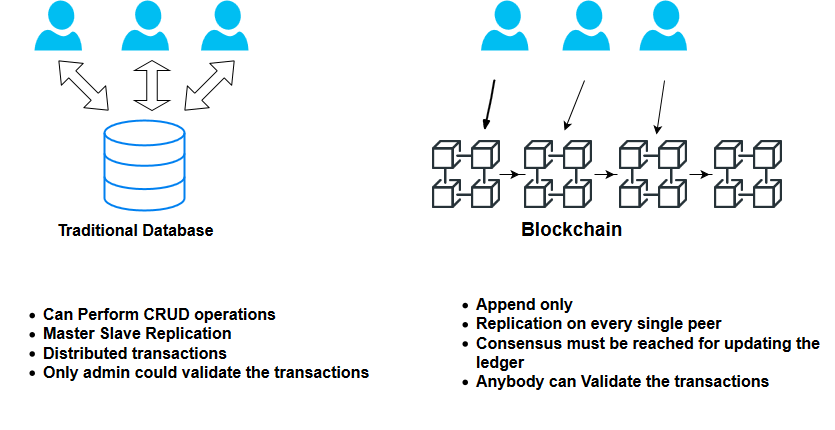
\includegraphics[width=15cm,height=10cm]{images/bcvsdb.png}
	\caption{Blockchain VS Traditional Database}
	\label{fig:bcvsdb}
	\end{figure}



\section{Hyperledger Fabric}
 
\subsection{Introduction}
Hyperledger Fabric is an Open-source permissioned Blockchain platform it was profounded under the Linux Foundation. Hyperledger Fabric became on of the most fastest growing project in the Linux Foundation. 
Hyperledger Fabric is the first platform that supports developing the smart contracts("chaincode") in general-purpose programming languages such as Java, Go and Node.js.
Furthermore, it's a permissioned blockchain in a simplified way this means the participants will be known to each other instead of being anonymous and fully untrusted. unlike permissionless which mainly relies on the miner to validate the transaction to relief the absence of trust. 
It provides a way to secure the interactions between different parties, which they not particularly trusting  each other having that it reinforces the trust between different entities.
Hypeledger Fabric is an enterprise distributed ledger based on GO programming language that uses smart contracts. 

Hyperledger Fabric came with a new concept that eliminates the mining concept, However it maintains all the characteristics of the blockchain, for instance, block immutability, order of operation determinism and the main benefits is the throughput of the system with huge number of transactions per minute by eliminating the concept of mining, also the consensus algorithm has the same properties as cryptocurrency blockchain. \\ 

Hyperledger is distributed by design there is no single point of failure or a single place that the information is stored.
all the participants are holding the same data, moreover, the data cannot be altered, thus hyperledger fabric reinforces the trust. 
Inside the blockchain, there is a ledger which stores every single operation occurred on the network. 
for example, imagine that there is a use case that we need to protect the copyright of some digital photos. and mistakenly we assigned a record of a photo to a wrong user and added the record to the ledger as a transaction. we couldn't delete this transaction, it will be always there and we have to assign the photo to the correct user. in essence, all the history of operations will be kept on the ledger, thus we could verify the all-time history of photos ownership by validating all the related transactions with the order of operation by replaying all the record inside the ledger you could find the latest world state,the world state or the final state of the data in our example the photo latest ownership will be the same amongst all network nodes, and due to the fact that the source of data is cryptographically signed that guarantees that the result of the data is the same trusted and unaltered. \\ 

Hyperledger Fabric could be integrated at any part of the network could serve the purpose publically or privately no matter it's physically located it will serve the purpose thanks to its flexibility t will fit and easily integrate within any system. \\ 


\subsection{Hyperledger Fabric Components} 

Hyperledger Fabric comprises of three main components:
\begin{itemize}
  \item Fabric Certificate Authority Fabric CA 
  \item Fabric Peer 
  \item Fabric Orderer 
\end{itemize} 


\textbf{ Fabric Certificate Authority (Fabric CA):} every single operation on hyperledger fabric must be signed with certificates no matter where the certificate came from if it is generated or purchased or generated from a trusted third party. Certificates are following X509 Standard and as mentioned there are many ways to generate certificates.
Fabric CA is a high-quality tool that pursues cryptographic standards to generate certificates these certificates are per user and attributes could be added while generating those certificates thus specific rules and permissions could be enforced per specific group of users. it is a place to generate certificates and  where the account would be created this process called enrollment you provide username and password and the fabric CA does all the magic. 
In addition fabric CA could be attached to an existing LDAP and all attributes would be fetched from there. 
by registering user and enroll them then provididing the certificate to SDK and the SDK signs all requests that will be executed inside hyperledger fabric. \\ 

\textbf{Peer:} is the place where the ledger blockchain is stored there could be more than one peer especially in production they contain the same ledger.  the request is sent from the SDK to peers, in order to do operations on the ledger like insert or query.  The main role of the peer is to endorse and update the ledger. all peers are synced automatically adding more peers in the network the other peer will automatically update the state of the newly joined peer, and this is facilitating the scalability of hyperledger fabric.  \\ 

\textbf{Orderer:} is coming into the heart of the consensus algorithm its main role is to provide order of operation before anything committed to the ledger it should be first validated and verified by the order and orderer creates the blocks so all transactions are stored into blocks and once blocks are full it will be sent to peers to be committed into the ledger. namely, the orderer is responsible for determining the order of operations.
There are several different implementations of ordering the first type is Solo which is mainly for development and this is only one instance if this instance fails all the operations for updating the ledger will fail, and the second type is Kafka which is used for production it's a distributed ordering service operation. \\

It's also worth mentioning \textbf{the channel} concept channels are a method developed in hyperledger fabric for data isolation More broadly it's a completely isolated instance of hyperledger fabric. every channel is completely independent and they never exchange data. when building network peers must be a part of the channel when creating peers, the peers should join a channel. with channel concept, the privacy and confidentiality of the data will be assured. the channel should be created and configured by a specific tool from hyper ledger fabric. in addition, one peer could be a part of different channels.  \\
 

\textbf{Chaincode} is a smart contract which is a program that reads and updates the ledger data, usually, all the business logic is written inside the chaincode. namely, the only way of interacting with the ledger will be only via the chaincode. 
The chaincode could be written in general purpose programming languages like Go, Java, and Javascript. There is no limitation on what could be done using chaincode it could have any desired complex business logic. \\

One important note that the chaincode must be apart of a channel inside one channel there could be as many as chaincodes. it could be possible to define all the business logic on one chaincode or split it amongst many chaincodes. 
The chaincode has to be installed and later instantiated. when writing chaincode it must be installed on every single peer that is a part of that channel this could be done using SDK or by using the peer itself. \\
 
Installing the chaincode on the peers is a must once it's the only way to interact with the ledger which resides on the peers. 
Once the chaincode is installed it should be then instantiated. 
Instantiating the chaincode will start a container that runs the chaincode while instantiating the chaincode the endorsement policy would be applied which will be responsible for validating and matching the rule on every single operation. For instance, applying a rule in a way  that for every transaction every peer must agree on adding the record otherwise the transaction will be rejected. \\  \\  \\ 
 
\textbf{Memebership Service Provider MSP}: is one of the most fundamental concepts of hyperledger fabric is a setup of cryptographical materials where the organizations will be defined. every single on hyperledger fabric must have its cryptographic certificates that define if a specific node belongs to specific organization generating the cryptographic material is trivial by hyperledger fabric tool cryptogen. 
The most essential part is that only peers that are part of the same MSP could communicate with each other. other peers couldn't the peer must be a part of the organization and this is defined by the peer's certificate later when configuring the channel all the public certificates will be shared on the configuration thus only the configured peer with a shared certificate could communicate and be a part of this channel. 

\textbf{The State Database:} In the blockchain concept, the state of the data would be tracked from the transactions history, for instance, assume that there is a simple balance transfer network. Person A sends 100 euros to person B and person C sends another 100 euros to person C. the current balance of person B should be 200 euros however the blockchain is just a serious of transaction in order to calculate the latest state of the accounts all transactions history should be reviewed and validated. thus for more efficient way hyper ledger fabric uses key-value store database to update the latest state of the data in an efficient way.
Chaincode invocations execute transactions against the current state data. To make these chaincode interactions extremely efficient, the latest values of all keys are stored in a state database. The state database is simply an indexed view into the chain?s transaction log, it can, therefore, be regenerated from the chain at any time. The state database will automatically get recovered (or generated if needed) upon peer startup before transactions are accepted.

State database options include LevelDB and CouchDB. LevelDB is the default state database embedded in the peer process and stores chaincode data as key-value pairs. CouchDB is an optional alternative external state database that provides addition query support when your chaincode data is modeled as JSON, permitting rich queries of the JSON content. See CouchDB as the State Database for more information on CouchDB.


\cleardoublepage

\subsection{Under The hood Hyperledger Fabric }

In this part, we will try to explain how hyperledger fabric works under the hood,
assume that we wanted to exchange the ownership of some assets, and The client wants to make a transaction, for example, adding data to the ledger. 
The first step is that the user has to register and enroll in the organization using fabric CA and get back the proper cryptographic materials that authorize him to interact with the network. Then the SDK will be responsible for preparing the transaction as a transaction proposal. This transaction will be sent to one or more peers. 
at this point the peer accepts this proposal and simulates it, the result of this simulation will be called read and write sets. at this phase, the ledger is not updated and the assets values remaining the same. 
The endorsing peers which are special kind of peers that its role is to verify and approve the transaction. this is will be done by validating the format and the signature of the transaction, and if the application user is authorized to make this transaction. 
then the peers are sending back those transaction responses to the SDK. the SDK collects all these transaction responses and signs it and send it to the orderer, the orderer node verifies the transaction signature and the endorsement policy. no matter if the transaction approved or rejected it will be stored on the blockchain, however, the state of the ledger will not be updated in case of the failure. in addition the order will verify the read and write sets collected from every single peer and makes sure they are all the same. 
Finally in case of the transaction is valid the orderer will send the transaction to the committing peers to be committed and updating the ledger.
\hyperref[fig:transactionflow]{Figure 2.2} depicts Hyperledger fabric transaction flow [1]. 
\begin{figure}[H]
	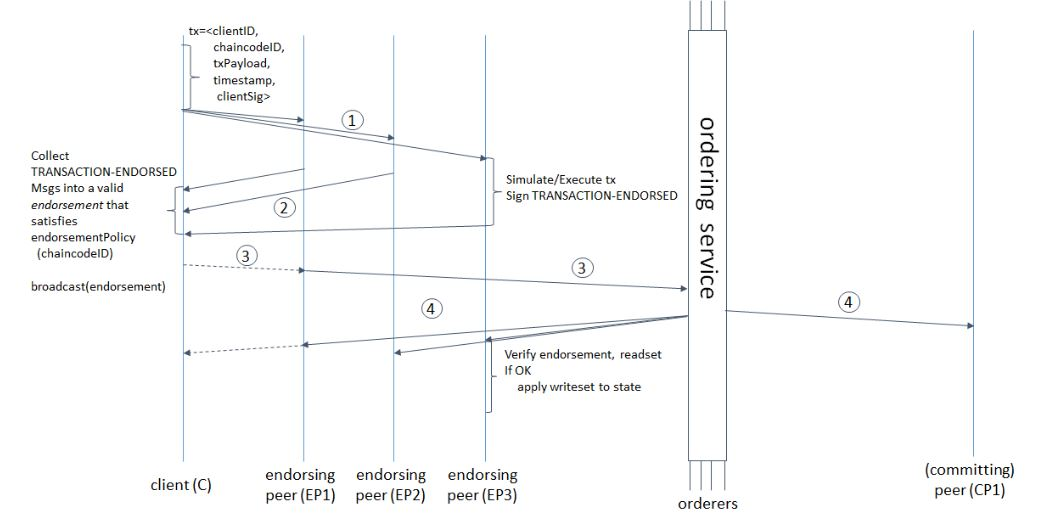
\includegraphics[width=15cm,height=10cm]{images/transactionflow.jpg}
	\caption{Hyperledger Fabric Transaction Flow Diagram}
	\label{fig:transactionflow}
	\end{figure}

 
 

 
 

 
 





 



 
  